\chapter{Solution d'administration à distance d'objets connectés}
\label{sec:content}

\section{Nécessité de cette solution}

La société Y3S développe toute sorte d'objets connectés comme des
centrales d'alarmes, sondes de relevé de température et tous hébergent
un serveur HTTP local pour sa gestion ou son utilisation.
Malheureusement pour accéder à son contenu local depuis internet il
faut ouvrir les ports et configurer les routeurs sur lequel j'ai
connecté l'objet. Pour les grandes entreprises ou collectivités il
n'est pas toujours possible d'effectuer ce genre de modification sur
leur architecture réseau à cause de problèmes de sécurité, de
compétence ou tout simplement parce que le nombre d'objets connectés
est trop important pour recevoir ces configurations manuellement pour
chaque unité.

Une autre solution consiste à développer un CLOUD sur lequel se
connectent tout les objets connectés et permettant aux utilisateurs
d'y accéder,par exemple, par l'intermédiaire d'un front-end
HTTP. Cette solution reste extrêmement coûteuse. En effet elle
nécessite de développer une solution CLOUD spécifique à chaque service
ou type d'objet connecté.

C'est donc dans cette optique que l'entreprise recherche une solution
qui permette de remplacer le CLOUD par une solution plus générique
donnant directement accès aux services locaux hébergés sur l'objet
connecté, réduisant ainsi les coût en développement et installation.

\section{Spécifications}

\subsection{Spécifications fonctionnelles}

Il est nécessaire de développer la solution en deux parties, le client
qui a installé sur l'objet et le serveur backend qui est en charge de
rendre l'objet connecté accessible sur internet. La solution doit être
capable de fournir un client ou un SDK à installer sur l'objet
connecté qui permet de se connecter au serveur backend de la
solution. Les principales fonctionnalités de la solution sont :
\begin{itemize}
\item produire un nom de domaine unique par objet connecté qui
  hébergent un serveur HTTP ;
\item gérer les déconnexions, reconnexions de l'objet connecté,
  pointer sur une page HTML d'erreur si on tente d'accéder au nom de
  domaine d'un objet déconnecté et fournir un nouveau nom de domaine
  unique si l'objet est resté déconnecté jusqu'à l'écoulement d'un
  délai prédéfini, sinon lui resservir le même nom de domaine ;
\item pouvoir se reconnecter automatiquement à un des serveurs s'il
  perd la connexion ;
\item la solution ne doit pas se contenter d'un seul protocole tel que
  le HTTP, mais doit pouvoir relayer n'importe quel protocole
  utilisant le TCP.
\end{itemize}

\subsection{Contraintes}

Le monde des objets connectés utilise des architectures de processeurs
spécifiques et variés. La solution cliente doit donc être
multi-plateforme, elle doit fonctionner sur UNIX, Windows, Android sur
des architectures x86/x64, ARM, MIPS. On doit pouvoir aussi
réimplémenter le client sur micro-contrôleur possédant une pile IP
parce qu'ils sont très utilisés dans le monde de l'industrie et donc
des objets connectés.

Certaine entreprise ont des pare-feux très restrictifs ne permettant la sortie que de certain protocole comme le HTTP et HTTPS respectivement sur le port 80 et 443.

\subsection{Spécifications techniques}

Pour répondre aux besoins de la solution, des choix techniques ont été
fait tout au long du développement du prototype de la solution. Au
début, Y3S m'a demandé de comparer les solutions existantes de Reverse
Tunneling, qui leur semblait être la technique la plus pertinente,
particulièrement si la solution utilise les websockets.

J'ai personnellement choisi de développer le client en C++, un langage
bas niveau orienté objet qui reste facile à compiler sur plusieurs
architectures. Le serveur a été développé en Node.js pour sa simplicité
de mise en place et de développement, sa scabilité et sa maintenance.

Pour résumer, voici les technologies techniques utilisées actuellement
sur le prototype à la fin de son développement, leur justification
d'utilisation suivra dans le rapport :
\begin{itemize}
\item reverse Tunneling en websocket : transfert de protocole TCP à
  travers n'importe quel routeur, pare-feu qui accepte le HTTP/HTTPS ;
\item C++ et socket natif : développement client ;
\item Node.js : développement serveur ;
\item Redis : base de données ;
\item OpenResty : proxy HTTP dynamique.
\end{itemize}

\section{Principe du Reverse Tunneling}

Pour illustrer le principe du reverse tunneling je vais me servir d'un
scénario. Imaginons que je souhaite atteindre le serveur HTTP d'Alice,
mais Alice est derrière un NAT qui bloque toute les connexions
entrantes sur son réseau. Malheureusement elle n'a pas la main sur son
routeur, ce qui empêche naturellement toute modification du
réseau. Par contre Bob a le contrôle de son réseau, qui accepte les
connexions entrantes sur sa machine, ce qui va me permettre de procéder
en sens inverse. C'est Alice que je souhaite joindre qui va créer une
connexion vers Bob que j'appelle le tunnel. En effet il suffit à Bob
d'écouter sur le port de son choix qu'Alice connaît, il attend
qu'Alice se connecte dessus et lui transmet sa requête HTTP. De son
côte Alice va recevoir la requête HTTP de Bob, qu'elle relaie à son
serveur HTTP et renvoie la réponse HTTP par cette même
connexion. C'est pour cela que cela s'appelle du reverse tunneling,
c'est notre cible qui est à l'initiative de la connexion, autrement
dit du tunnel.
\begin{figure}[htp]
  \centering
  \begin{pspicture}(0,0)(14,6)
    \psset{framearc=0.2}
    \psframe(0,0)(5,3.5)
    \uput[u](2.5,3.5){Alice}
    \psframe(0.5,0.5)(2,2)
    \rput(1.25,1.25){%
      \begin{tabular}{c}
        HTTP\\
        Server
      \end{tabular}%
    }
    %
    \psframe(9,0)(14,3.5)
    \uput[u](11.5,3.5){Bob}
    \psframe(13.5,0.5)(12,2)
    \rput(12.75,1.25){%
      \begin{tabular}{c}
        WWW
      \end{tabular}%
    }
    %
    \pspolygon[fillstyle=solid, fillcolor=cyan]
      (3.5,0.5)(3.5,2)(4.5,2)(4.5,1.8)(4.7,1.6)
      (9.3,1.6)(9.5,1.8)(9.5,2)(10.5,2)
      (10.5,0.5)(9.5,0.5)(9.5,0.7)(9.3,0.9)
      (4.7,0.9)(4.5,0.7)(4.5,0.5)
      \uput[u](7,1.6){Tunnel}
    %
    \pspolygon[fillstyle=solid, fillcolor=white]
      (2,1.25)(2.5,1.75)(2.5,1.4)(11.5,1.4)(11.5,1.75)
      (12,1.25)(11.5,0.75)(11.5,1.1)(2.5,1.1)(2.5,0.75)
      \rput(7,1.2){\scriptsize HTTP Request}
  \end{pspicture}
  \caption{Principe du reverse tunneling}
  \label{fig-tunneling}
\end{figure}

\section{Comparaison de solution de reverse tunnel}

Après quelques jours de recherche, j'ai retenu trois solutions de
reverse tunnel :
\begin{itemize}
    \item OpenSSH ;
    \item Etherws ;
    \item Node Reverse Wstunnel.
\end{itemize}

\subsection{OpenSSH}

OpenSSH est une suite d'outils SSH libres mettant à disposition un
client et server SSH très complet. Or le SSH permet d'initialiser un
tunnel directement avec une commande SSH. Pour en revenir sur notre
scénario précédent. Bob installe un serveur SSH sur sa machine (sur le
port 22), toujours accessible de l'extérieur par le nom de domaine
bob.fr et rajoute sur son serveur SSH l'utilisateur Alice. Elle va s'y
connecter en précisant qu'elle ouvre un tunnel inverse de son port 80
sur lequel écoute son serveur HTTP, jusqu'au port de son choix par
exemple le 8080. Bob peut désormais accéder au serveur d'Alice en
remontant le tunnel par l'adresse \url{http://localhost:8080}.

L'action se résume par cette unique ligne de commande qu'Alice exécute
sur sa machine :
\begin{lstlisting}[language=bash]
  $ ssh -NR 8080:localhost:80 alice@bob.fr
\end{lstlisting}%$

Bien évidemment cela fonctionne pour n'importe quel service en TCP, il
suffit juste de choisir le bon port.

Avantages :
\begin{itemize}
\item facile à mettre en place ;
\item automatiquement sécurisé.
\end{itemize}

Inconvénients :
\begin{itemize}
\item les micro-contrôleur ne possèdent pas de client SSH, en
  développer un serait périlleux ;
\item pour chaque port ouvert il faut une nouvelle connexion SSH ;
\item un serveur SSH n'est pas optimisé pour maintenir une centaine de
  connexion permanente ;
\item le port d'entrée et sortie du tunnel est choisi par le client ;
\item puisque que c'est du SSH, le port du serveur tunnel y est aussi.
\end{itemize}

\subsection{Etherws}

Etherws est un mini VPN utilisant des websockets comme tunnel, il est
entièrement développé en python. La configuration se fait en deux
étapes : création de l'interface virtuelle en TUN/TAP avec l'adressage
de l'IP virtuelle puis connexion au serveur (toujours celui de Bob qui
est le seul à disposer d'un nom de domaine public). Le fait d'utiliser
une interface virtuelle permet d'utiliser tous les ports à la fois
sans en préciser un en particulier qui doit être relié à un autre
distant sur la machine de Bob.

Dans notre cas Alice va choisir d'appeler son interface virtuel \og
etherws0 \fg{} avec l'IP \og 10.0.2.8 \fg{} et se connecter sur le
serveur etherws de Bob (en 80). Pour accéder au serveur HTTP d'Alice,
Bob doit remonter le tunnel en passant par l'IP virtuel d'Alice, soit
comme cela \url{http://10.0.2.8:80}.

Commande nécessaire à la création du tunnel :
\begin{lstlisting}[language=bash]
  etherws sw
  etherws ctl addport tap ethws0
  etherws ctl setif --address 10.0.2.8 --netmask 255.255.255.0 1
  etherws ctl addport client ws://bob.fr/
\end{lstlisting}

Avantages :
\begin{itemize}
\item utilise les websockets ;
\item peut être sécurisé en SSL/TLS.
\end{itemize}

Inconvénients :
\begin{itemize}
    \item monte une interface virtuelle ;
    \item l'IP virtuelle est choisi par le client ;
    \item tous les clients peuvent communiquer ensemble par le réseau
      virtuel ;
    \item portage difficile, voir impossible sur micro contrôleur.
\end{itemize}

\subsection{Node Reverse Wstunnel}

Node Reverse Wstunnel est un tunnel inversé développé en javascript
avec Node.js, utilisant les websockets. Il s'utilise sur le même
principe que le tunnel inversé SSH mais en passant par un tunnel
websocket au lieu d'un tunnel SSH. Bob lance sur sa machine le serveur
tunnel inversé en 80 (avec node) et Alice s'y connecte avec le client
fourni en précisant les deux ports qu'elle veut relier.

Si on reprend la même configuration que pour le tunnel SSH, la
commande qu'Alice doit exécuter est :
\begin{lstlisting}[language=bash]
  $ ./wstt.js -r 8080:localhost:80 ws://bob.fr/
\end{lstlisting}%$

Bob peut donc accéder au serveur HTTP d'Alice en se connectant en
\url{http://localhost:8080}.

Avantages :
\begin{itemize}
    \item Utilise les websockets.
    \item Peut être sécurisé en SSL/TLS.
\end{itemize}

Inconvénients :
\begin{itemize}
    \item Le port d'entrée et sortie du tunnel est choisi par le client.
\end{itemize}

\subsection{Choix final}

Finalement j'ai décidé avec mon maître de stage de choisir la solution
de reverse tunneling en Node.js en websocket, mais en reprogrammant le
client en C++ parce que le Node.js n'est pas portable sur toute les
versions d'ARM. Le serveur restera en Node.js mais sera réécrits pour
mieux répondre à nos besoins, c'est en effet une technologie
facilement maintenable pour développer un serveur websocket
évolutif. L'architecture de base de Node Reverse Wstunnel est la seule
chose conservée dans son intégrité.

\section{Proxy HTTP dynamique}

J'ai trouvé comment accéder à une machine distante sans modifier son
NAT ou connaître son IP. Cependant notre objectif était d'accéder à
plusieurs machines (objets connectés) à travers un nom de domaine
unique pour chacune. Si je reprends l'exemple précédent d'Alice et
Bob, Alice fait tourner son serveur HTTP sur le port 80, en se
connectant au serveur wstunnel de Bob elle a demandé à relier son port
80 avec le port 8080 de Bob. Ainsi depuis internet, si on se connecte
en \url{http://bob.fr:8080} on accède au serveur HTTP d'Alice, car Bob
possède un nom de domaine qui pointe sur l'IP fixe de sa machine. Cela
fonctionne parfaitement sauf qu'on voulait un nom de domaine sans
devoir préciser le port, certes on pourrait déplacer le serveur
wstunnel sur le port 8080 et remettre le tunnel du port 80 d'Alice au
port 80 de Bob comme cela le nom de domaine serait bob.fr tout
simplement. Mais qu'arriverait il si je souhaite rajouter une ou dix
autres machines dans le même cas qu'Alice ? Il me faudrait bien
utiliser des ports autre que le 80.

C'est pour résoudre ce problème que j'ai dû installer un proxy
HTTP. Celui-ci est en fait un serveur HTTP qui va rediriger une
requête ou une réponse HTTP sur un autre port en fonction du nom de
domaine. Quand je rentre un nom de domaine dans un navigateur,
celui-ci va résoudre le nom de domaine en IP et envoyer une requête
HTTP sur cette IP, port 80 par défaut. C'est grâce à la requête HTTP
que le proxy peut connaître le serveur cible sur lequel rediriger la
requête. En effet une requête HTTP contient un champs \og Host \fg{}
qui contient le nom de domaine que l'utilisateur a saisi dans le
navigateur, le proxy redirige donc en fonction de ses configurations
sur tel ou tel port la requête et la réponse HTTP.

Dans ce cas Bob peut configurer son proxy HTTP qui écoute sur le port
80 pour qu'il redirige le nom de domaine \og alice.bob.fr \fg{} en \og
localhost:8080 \fg{} (le serveur wstunnel est sur un autre port
disponible).

Exemple de requête HTTP :
\begin{lstlisting}[language=bash]
  GET / HTTP/1.1
  Host: alice.bob.fr
\end{lstlisting}

Malheureusement la plupart des proxy HTTP sont configurables à
l'arrêt, ce qui veut dire que si je veux rediriger d'autre serveur
HTTP comme Alice, je dois éditer les configurations du proxy et
redémarrer les services, le tout manuellement. C'est tout simplement
impossible pour nos objectifs lorsqu'on doit rediriger des centaines
de noms de domaines uniques pour autant d'objets connectés. Il m'a
fallu rechercher un solution dynamique à notre problème.

OpenResty est un serveur, proxy HTTP basé sur Nginx, qui a la
particularité d'être très modulable grâce à ses nombreux modules
configurables et à la possibilité d'exécuter des scripts LUA lorsque
l'on reçoit une requête HTTP. LUA est un langage de scripting très
léger et facile à embarquer. Avec OpenResty j'ai pu écrire une
configuration de proxy qui lorsque qu'il reçoit une requête, recherche
\og Host \fg{} dans notre base de données et si ce nom de domaine
existe dans la base, alors redirige la requête vers l'IP et port
associés. Tout cela est possible grâce à un script LUA qui se connecte
à la base de données, de plus je peux rajouter des noms de domaines à
rediriger dans la base de données sans à devoir redémarrer le
proxy. OpenResty m'a donc permis de créer un proxy HTTP dynamique.

\section{Base de données Redis}

Pour faire fonctionner l'ensemble de la solution, il a fallu faire le
choix d'une base de données centrale qui ferait le lien entre le proxy
HTTP dynamique et le serveur wstunnel en Node.js, mais aussi avec la
futur partie front-end, en charge d'afficher la liste des ports
redirigés pour chaque client et le nom de domaine unique si c'est un
port 80 ou 443. J'ai fait le choix d'utiliser Redis, qui est une base
de données No-SQL dont la particularité est de stocker tout son
contenu dans la mémoire vive.

Redis utilise des structures de données très simple comme des listes,
des ensembles, des tableaux associatifs ou même des ensembles
triés. Elle peut stocker des dizaines de millions de clefs et valeurs
dans à peine 100 MiO de RAM. Son protocole de communication, ses
structures et son stockage en RAM ont fait d'elle une base de données
extrêmement rapide, c'est justement ce qu'il faut pour que notre proxy
HTTP dynamique réponde le plus rapidement possible aux requêtes. Une
petite fonctionnalité de Redis permet aussi de rajouter un délai
d'expiration sur certaines valeurs stockées avant leur suppression,
cela c'est avéré pratique pour supprimer automatiquement les noms de
domaines et ports qui n'étaient plus utilisés par l'objet connecté qui
s'est justement déconnecté. Une fonctionnalité qui permet donc de
libérer les ports non utilisés et gagner en capacité. Par contre si
l'objet connecté se reconnecte avant la fin du délai, alors il
conserve son port et son nom de domaine alloué. Si jamais le serveur
tombe et que l'on perd les données Redis stockés dans la RAM, cela
n'est pas très grave, les données en questions sont les ports et les
noms de domaines qui étaient utilisés par le serveur tunnel, mais si
Redis est tombé alors le serveur tunnel l'est aussi donc tout ses
ports utilisés ne sont plus du tout d'actualités.

\section{Modification et Re-developpement du Tunnel WebSocket}

\subsection{WebSocket}

Le websocket est un protocole réseau standard du Web visant à créer
une communication full-duplex sur une connexion HTTP, donc en TCP. Ce
protocole a été normalisé dans la RFC 6455, son but est de pouvoir
établir des communications bidirectionnelles avec un long temps de vie
entre le client et serveur HTTP afin de notifier le client d'un
changement d'état du serveur ou même d'envoyer des données ponctuelles
du serveur au client.

Pour initialiser une connexion websocket il faut envoyer une requête
HTTP spécifique au serveur qu'on appelle le \og Handshake \fg{} au
quel le serveur doit répondre avec une réponse HTTP. Ensuite à partir
de cette échange, la connexion HTTP passe en connexion websocket.

Exemple de requête handshake :
\begin{lstlisting}[language=bash]
  GET /chat HTTP/1.1
  Host: example.com:8000
  Upgrade: websocket
  Connection: Upgrade
  Sec-WebSocket-Key: dGhlIHNhbXBsZSBub25jZQ==
  Sec-WebSocket-Version: 13
\end{lstlisting}

Exemple de réponse handshake :
\begin{lstlisting}[language=bash]
  HTTP/1.1 101 Switching Protocols
  Upgrade: websocket
  Connection: Upgrade
  Sec-WebSocket-Accept: s3pPLMBiTxaQ9kYGzzhZRbK+xOo=
\end{lstlisting}

Lors du handshake le client passe dans la requête HTTP le champs \og
Sec-WebSocket-Key \fg{} qui contient une clef générée aléatoirement
par le client et cryptée en base~64. Le serveur doit hacher en SHA1 la
concaténation de cette clef avec une chaîne de caractères prédéfinie
dans la RFC~6455 et convertir la sortie en base~64, ce qui correspond
dans la réponse au champs \og Sec-WebSocket-Accept \fg{}. Le client
doit ou peut réaliser la même opération pour vérifier qu'il communique
bien avec un serveur websocket et non un proxy qu'il lui renverrait un
simple cache.

La suite de la communication est entièrement basée sur des trames
websocket binaires, rythmées par des échanges de trames de contrôle
ping et pong dit \og battement de cœur \fg{}, pour avoir la certitude
que la connexion est toujours active. Je ne vais pas détailler
d'avantage les trames websocket car cela est peu utile et très
spécifique, il suffit de lire la RFC 6455, je rajouterai seulement que
le webscoket permet d'envoyer deux types de données, du texte brute
UTF-8 et du binaires.

\begin{figure}[htp]
\centering
\begin{lstlisting}[gobble=0, numbers=left, frame=l,
  basewidth={0.55em, 0.4em}]
 0               1               2               3              
 0 1 2 3 4 5 6 7 0 1 2 3 4 5 6 7 0 1 2 3 4 5 6 7 0 1 2 3 4 5 6 7
+-+-+-+-+-------+-+-------------+-------------------------------+
|F|R|R|R| opcode|M| Payload len |    Extended payload length    |
|I|S|S|S|  (4)  |A|     (7)     |             (16/64)           |
|N|V|V|V|       |S|             |   (if payload len==126/127)   |
| |1|2|3|       |K|             |                               |
+-+-+-+-+-------+-+-------------+ - - - - - - - - - - - - - - - +
 4               5               6               7              
+ - - - - - - - - - - - - - - - - - - - - - - - - - - - - - - - +
|     Extended payload length continued, if payload len == 127  |
+ - - - - - - - - - - - - - - - +-------------------------------+
 8               9               10              11             
+ - - - - - - - - - - - - - - - +-------------------------------+
|                               |Masking-key, if MASK set to 1  |
+-------------------------------+-------------------------------+
 12              13              14              15
+-------------------------------+-------------------------------+
| Masking-key (continued)       |          Payload Data         |
+-------------------------------- - - - - - - - - - - - - - - - +
:                     Payload Data continued ...                :
+ - - - - - - - - - - - - - - - - - - - - - - - - - - - - - - - +
|                     Payload Data continued ...                |
+---------------------------------------------------------------+
\end{lstlisting}
\caption{Trame WebSocket}
\end{figure}

\subsection{Fonctionnement}

Pour expliquer le principe de fonctionnement du tunnel en websocket
(qui sera toujours en mode \og reverse \fg{}) qu'on appellera plus
facilement le tunnel, sans pour l'instant y ajouter le proxy HTTP
dynamique, je vais en redéfinir les acteurs, il y en a trois
principaux :
\begin{description}
\item[Le serveur] C'est le serveur websocket principal qui pilote tout
  le tunnel, son IP est donc connu et publique. Il est connectés à la
  base de données Redis, sur laquelle il stock les ports alloué et
  connexions courantes.
\item[Le client] C'est la machine ou objet connecté souhaitant rendre
  accessible un de ses serveurs au public, dans notre cas se sera un
  serveur HTTP.
\item[Le navigateur] C'est un utilisateur externe qui veut accéder au
  service du client, dans notre cas il fait une requête HTTP sur un
  port défini du serveur websocket.
\end{description}

Pour faire fonctionner le tunnel il faut au minimum deux connexions
websockets, la première est le websocket de contrôle, il sert à
initialiser et avertir le client d'une nouvelle connexion du
navigateur. Dans le handshake du websocket de contrôle, il faut passer
dans l'URL les paramètres suivant : le nom du client et les ports
qu'il souhaite faire passer. Le serveur va allouer au client un port
disponible sur sa machine ou bien lui donner un port qu'il a déjà
utilisé lors de sa précédente connexion mais qui n'a pas encore
expiré. Le serveur va monter ce nouveau port alloué comme serveur TCP
et y attendre une connexion. Bien sur si un client avec le même nom
est déjà connecté la connexion sera refusée. C'est ce que j'appelle la
phase d'initialisation du tunnel. Maintenant un navigateur qui connaît
le port alloué au client sur le serveur va se connecter dessus et y
effectuer une requête HTTP. Le serveur va accepter la connexion (étant
donné qu'une requête HTTP utilise le TCP), il va mettre en attente le
navigateur, étiqueter cette connexion avec un ID unique et envoyer un
message sur le websocket de contrôle au client associé à ce port
alloué. Ce message est très simple, il contient simplement le port qui
a été associé à cette allocation de port lors de la phase
d'initialisation du tunnel, soit le port 80 pour un serveur HTTP et
l'ID de la connexion du navigateur. En recevant ce message par le
websocket de contrôle le client va créer un nouvelle connexion
websocket sur le serveur (que j'appelle le websocket de transfert)
mais cette fois l'URL du handshake contiendra en paramètre l'ID
associé à la connexion du navigateur. Il va aussi créer une connexion
locale vers son serveur HTTP et la relier au nouveau websocket de
transfert, parce que le message reçu indiquait une redirection sur le
port 80. Ainsi quand serveur recevra la connexion websocket, il saura
exactement que c'est un websocket de transfert grâce à l'ID dans l'URL
associé à la connexion du navigateur en cours. Maintenant que le
tunnel est complètement formé le serveur va rediriger la requête du
navigateur dans le websocket de transfert associé en mode binaire qui
va lui même la rediriger côté client au serveur HTTP. Celui-ci va
répondre en envoyant une réponse HTTP qui va faire le chemin
inverse. Une fois la réponse arrivée jusqu'à son destinataire, le
navigateur va fermer la connexion TCP, ce qui va fermer également le
websocket de transfert associé à cette connexion ainsi que la
connexion locale au serveur HTTP du client. Seuls resteront le
websocket de contrôle et le serveur TCP montés sur le port alloué qui
attendront une nouvelle connexion d'un navigateur. Comme les
connexions du navigateur sont étiquetées d'un ID unique, plusieurs
connexions peuvent être traitées à la fois ce qui entraîne autant de
websocket de transfert que de connexions des navigateurs, voilà
pourquoi le websocket de contrôle n'est là que pour avertir des
nouvelles connexions et ne fait pas aussi le transfert des
requêtes. Si c'était le cas il y aura trop d'attente entre chaque
requête. Lorsque que le client va fermer la connexion du websocket de
contrôle alors le serveur TCP associé au port alloué au client va se
fermer et le port prendra un délai d'expiration dans la base de
données Redis.
\begin{figure}[htp]
  \centering
  \begin{pspicture}(0,0)(15,8.5)
    \psset{framearc=0.2, tbarsize=6pt 15, arrowsize=3pt 4, labelsep=2pt}
    \uput[u](2,8){Alice}
    \psframe(0,0)(4,8)
    \psline{-|}(1,0.5)(1,7)\uput[u](1,7){HTTP}
    \psline{-|}(3,0.5)(3,7)\uput[u](3,7){WS Client}
    %
    \uput[u](8.5,8){Bob}
    \psframe(7.5,0)(9.5,8)
    \psline{-|}(8.5,0.5)(8.5,7)\uput[u](8.5,7){WS Server}
    %
    \psframe(13,0)(15,8)
    \psline{-|}(14,0.5)(14,7)\uput[u](14,7){Navigator}
    %
    % Flèches
    \psline{->}(1,1)(3,1)
    \psline{->}(3,2)(1,2)
    \uput[u](2,2){Request}
    \uput[u](2,1){Response}
    %
    \psline{->}(3,1)(8.5,1)
    \uput[u](5.75,1){Transfert Response}
    \psline{->}(8.5,2)(3,2)
    \uput[u](5.75,2){Transfert Request}
    \psline{->}(3,3)(8.5,3)
    \uput[u](5.75,3){Transfert WS}
    \psline{->}(8.5,4)(3,4)
    \uput[u](5.75,4){\begin{tabular}[b]{c}Message\\New Connection\end{tabular}}
    \psline{->}(3,6)(8.5,6)
    \uput[u](5.75,6){Control WS}
    %
    \psline{->}(8.5,1)(14,1)
    \uput[u](11.25,1){HTTP Response}
    \psline{->}(14,5)(8.5,5)
    \uput[u](11.25,5){HTTP Request}
  \end{pspicture}
  \caption{Diagramme de séquence}
  \label{fig-sequence}
\end{figure}

\subsection{Répartition de la charge}

Cette solution serveur tunnel est prévue pour accueillir des centaines
ou des milliers de client. Chaque client doit au minimum maintenir
avec le serveur une connexion websocket de contrôle permanente, parce
qu'un serveur ne doit en principe jamais s'éteindre. Ce qui pose un
problème de capacité machine, en effet une machine physique ne peut
ouvrir qu'un certain nombre de ports au maximum. Notre serveur tunnel
doit donc être multiplié en plusieurs grappes.

Pour palier à ce problème j'ai ajouté une petite implémentation sur le
serveur tunnel. Chaque serveur dispose d'une IP et d'un compteur de
client dans la base de données Redis. Quand un client ce connecte sur
un serveur, celui-ci va faire un requête à Redis pour trier et
sélectionner l'IP qui possède le moins de clients grâce au compteur de
chaque serveur. Si l'IP qu'il obtient est la sienne, alors le serveur
tunnel accepte la connexion websocket de contrôle et incrémente son
compteur, sinon il retourne au client une réponse HTTP de code 302
avec en location l'IP, ce qui signifie une redirection HTTP sur cette
IP, ne pas oublier que le websocket est construit sur un serveur HTTP
à l'aide d'une requête handshake donc c'est totalement possible. Le
client va devoir refaire une connexion websocket sur l'IP de
redirection, jusqu'à obtenir un serveur qui l'accepte.

\section{Le client}

\subsection{Toolchain}

j'ai choisi de développer le client en C++, ce qui m'a demandé de
compiler le client pour chaque architectures. J'ai donc dû faire de la
compilation croisée en utilisant une chaîne de compilation (\og
toolchain \fg{}) spécifique, c'est-à-dire que j'ai compilé sous UNIX
mais en utilisant un compilateur qui a compilé mes sources dans un
format d'exécutable qui pouvait être exécuté sur le système
d'exploitation et architectures cible. Toute ces chaînes de
compilations avaient en commun d'être basées sur le compilateur
GCC. J'ai utilisé ces chaînes de compilation pour ces cibles précises :
\begin{itemize}
\item arm-linux-gnueabi : pour ARM (Android, Raspbian et autre kernel
  UNIX) ;
\item mips-openwrt-linux-uclibc : pour MIPS (Arduino Yun) ;
\item x86\_64-w64-mingw32 : pour Windows x64 ;
\item i686-w64-mingw32 : pour Windows x32, particulièrement Windows XP.
\end{itemize}

Certaines chaînes de compilation ont dû elles-mêmes être compilées pour
être exécutées sur ma version de GNU/Linux de développement.

\subsection{Socket natif}

Pour m'assurer d'être entièrement portable j'ai essayé de ne pas
utilisé de bibliothèque tiers. J'ai seulement utilisé une bibliothèque
de cryptographie pour pouvoir vérifier la validité de la clef du
hanshake websocket renvoyé par le serveur. Elle m'a permet d'utiliser
le SHA1 et la base~64, mais à cause de cela, je l'ai recompilée à la
main, en réécrivant les makefiles pour chaque architecture ce qui
était plus tôt fastidieux.

Puisque que je n'utilisais pas de bibliothèque réseau, j'ai
directement utilisé les sockets natifs à chaque système
d'exploitation. Les sockets permettent de réaliser facilement des
connexions TCP ou UDP ou d'ouvrir un port pour y attendre des
connexions. Ce sont des fonctionnalités réseau assez bas niveau, j'ai
dû écrire par dessus ma propre implémentation d'un client websocket et
d'un proxy de redirection de flux. Malheureusement les sockets sont
encore une fonctionnalité pas complètement portable. En effet
certaines fonctionnalités liées aux sockets sont différentes sur UNIX
et sur Windows, voir même inexistante sur d'autres systèmes
d'exploitation.

Pour palier à ce problème, j'ai utilisé des macros conditionnelles en
C, pour que mon compilateur me compile une partie de mon code source
uniquement pour un systèmes d'exploitation et pas pour les
autres. Pour les fonctionnalités inexistantes, je n'ai eu d'autre
choix que de les remplacer par d'autre plus anciennes.  C'est le cas
avec Windows XP qui n'avait pas certaines fonctions essentielles de
gestion de socket existantes sur Windows Vista, Seven ou 10.

Étant donné que le client doit pouvoir lire plusieurs sockets en même
temps quand, par exemple, plusieurs connexions websocket de transfert
sont créées, j'ai utilisé des sockets en mode asynchrone, c'est-à-dire
qui ne bloquaient pas le processus quand ils n'avaient rien à recevoir
d'une connexion. Cela nécessite d'utiliser aussi des fonctions
systèmes de gestion de sockets qui ne consomment pas de CPU quand il
n'y a rien à recevoir. J'ai par exemple utilisé \og poll \fg{}, appelé
\og WSAPoll \fg{} sous Windows, qui servait à me signaler quand il y
avait un socket possible à lire parmi un tableau de sockets. Sous
Windows XP \og WSAPoll \fg{} n'existe pas, j'ai utilisé une autre
version plus ancienne appelé \og select \fg{}. Toute ces modifications
spécifiques ont pu être possibles sur le même code source en utilisant
les macros conditionnelles.

\subsection{Diagramme de classe}
\begin{figure}[htp]
  \centering
  \begin{pspicture}(0,0)(14,7)
    \def\Short(#1)#2{%
      \rput(#1){
        \psframe(0,0)(2,2)
        \rput(1,1){#2}
      }
    }%
    \def\LG(#1)(#2){%
      \psline(#1)(#2)
      \rput(#1){\pspolygon*(0,0)(0.25,0.15)(0.5,0)(0.25,-0.15)}
    }
    \def\lB(#1)(#2){%
      \psline(#1)(#2)
      \rput(#1){\pspolygon[fillstyle=solid](0,0)(0.15,0.25)(0,0.5)(-0.15,0.25)}
    }
    \def\lBD(#1)(#2){%
      \psline(#1)(#2)
      \rput{45}(#1){\pspolygon[fillstyle=solid](0,0)(0.15,0.25)(0,0.5)(-0.15,0.25)}
    }
    \def\tG(#1)(#2){%
      \psline(#1)(#2)
      \rput(#1){\pspolygon[fillstyle=solid](0,0)(0.4,0.25)(0.4,-0.25)}
    }
    \def\tH(#1)(#2){%
      \psline(#1)(#2)
      \rput(#2){\pspolygon[fillstyle=solid](0,0)(0.25,-0.4)(-0.25,-0.4)}
    }
    \def\tB(#1)(#2){%
      \psline(#1)(#2)
      \rput(#1){\pspolygon[fillstyle=solid](0,0)(0.25,0.4)(-0.25,0.4)}
    }
    %
    \psset{framearc=0.2}
    \Short(0,4){Manager}
    \Short(4,4){TCP}
    \Short(8,4){ITCP}
    \Short(12,4){Control}
    \Short(4,0){WS}
    \Short(8,0){Node}
    %
    \LG(2,5)(4,5)
    \LG(6,5)(8,5)
    \tG(10,5)(12,5)
    \tH(5,2)(5,4)
    \tH(9,2)(9,4)
    \psline(13,6)(13,7)(1,7)\lB(1,6)(1,7)
    \lBD(8.07,1.93)(5.93,4.07)
  \end{pspicture}
  \caption{Diagramme de classe simplifié du client}
  \label{fig-classe-client}
\end{figure}

\section{Vue d'ensemble de la solution}

\begin{figure}[htp]
  \centering
  \begin{pspicture}(0,0)(12,11)
    \def\Long(#1)#2{%
      \rput(#1){
        \psframe(0,0)(3,2)
        \rput(1.5,1){#2}
      }
    }%
    \def\Short(#1)#2{%
      \rput(#1){
        \psframe(0,0)(2,2)
        \rput(1,1){#2}
      }
    }%
    \psset{framearc=0.2}
    %%%
    \Long(0,7.5){IoT}
    \Long(0,1.5){Navigator}
    \Short(4,1.5){Proxy}
    \Short(4,7.5){Proxy}
    \Short(7,0){Front-End}
    \Short(7,3){%
      \begin{tabular}{@{}c@{}}
        Open\\Resty
      \end{tabular}
    }
    \Short(7,6){%
      \begin{tabular}{@{}c@{}}
        Server\\WS
      \end{tabular}
    }
    \Short(7,9){%
      \begin{tabular}{@{}c@{}}
        Server\\WS
      \end{tabular}
    }
    \Short(10,7.5){Redis}
    % Fléèches
    \psset{linewidth=1.5pt, arrowsize=2pt 3}
    \psline{<->}(3,2.5)(4,2.5)
    \psline[linecolor=green]{<->}(3,8.5)(4,8.5)
    \psline{<->}(6,2.5)(7,1)
    \psline{<->}(6,2.5)(7,4)
    \psline[linecolor=green]{<->}(6,8.5)(7,7)
    \psline[linecolor=green]{<->}(6,8.5)(7,10)
    \psline[linecolor=red]{<->}(9,1)(11,1)(11,7.5)
    \psline[linecolor=red]{<-}(9,4)(11,4)
    \psline[linecolor=blue]{<->}(9,4.25)(9.5,4.25)(9.5,9.25)(9,9.25)
    \psline[linecolor=blue]{<-}(9,7)(9.5,7)
    \psline[linecolor=red]{<->}(9,7.25)(10,8.5)
    \psline[linecolor=red]{<->}(9,10)(10.1,9.4)
  \end{pspicture}
  \caption{Représentation de l'architecture serveur}
  \label{fig-ensemble}
\end{figure}
\section{Implémentation sur micro-contrôleur}

En fin de stage, on m'a demandé d'essayer d'implémenter le client
tunnel sur un micro-contrôleur qui intègre la WIFI. Le choix s'est
porté sur un ESP8266 modèle ESP-01, c'est un module WIFI IoT de la
marque Expressif basé sur un micro-contrôleur Xtensa Tensilica,
cadencé à 80\,MHz, accompagné de 512K de mémoire FLASH pour une
alimentation total de 3,3\,V. Ce module dispose de sa chaîne de
compilation du nom de \og xtensa-lx106-elf \fg{}, elle aussi basée sur
GCC, ainsi que d'un SDK fourni par Espressif pour développer un
firmware à l'ESP8266 en C.

\begin{figure}[htp]
  \centering
  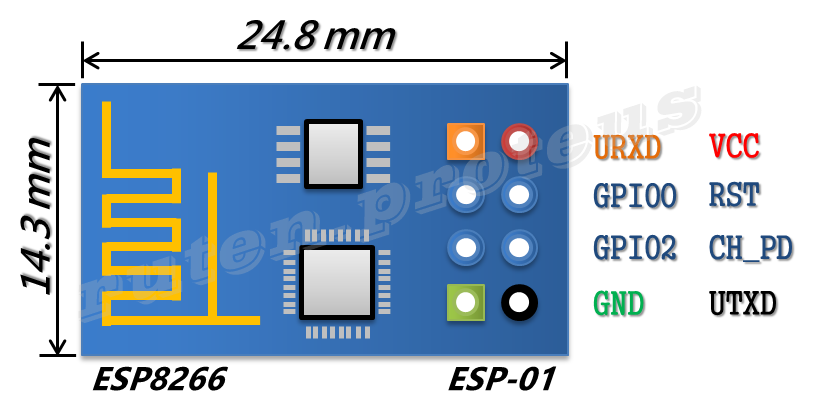
\includegraphics[width=12cm]{images/esp}
  \caption{ESP8266 ESP-01}
  \label{fig:une-autre-image}
\end{figure}

Il m'a fallu décortiquer le SDK pour réimplémenter une version
spécifique minimal du client en C. Cette version expérimentale ne
pouvait ouvrir qu'un seul websocket de transfert à la fois et le
contenu de la page WEB était directement stocké en dur dans le
programme du microcontrôleur. Une fois le programme compilé en
binaire, il fallait le flasher dans la mémoire flash du
micro-contrôleur en UART (alias Serial), à l'aide d'un adaptateur UART
en USB, par exemple de la marque FTDI.

\begin{figure}[htp]
  \centering
  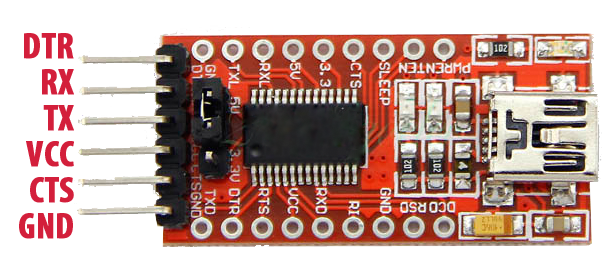
\includegraphics[width=12cm]{images/ftdi}
  \caption{FTDI FT232RL USB to TTL Serial Adapter}
  \label{fig:une-autre-image}
\end{figure}

Ce petit prototype sur micro-contrôleur a tout de même était capable
de se connecter au serveur par l'intermédiaire de notre WIFI (SSID et
mot passe codé en dur dans le programme), son nom de domaine unique
généré par le serveur pointait sur la page WEB stocké sur l'ESP,
permettant d'allumer/éteindre une LED branchée au micro-contrôleur sur
le GPIO2 à l'aide d'un bouton HTML.

%%% Local Variables: 
%%% mode: latex
%%% TeX-master: "isae-report-template"
%%% End: 
